\documentclass{article}
\usepackage{amssymb,amsmath}
\usepackage{ifxetex,ifluatex}
\ifxetex
  \usepackage{fontspec,xltxtra,xunicode}
  \defaultfontfeatures{Mapping=tex-text,Scale=MatchLowercase}
\else
  \ifluatex
    \usepackage{fontspec}
    \defaultfontfeatures{Mapping=tex-text,Scale=MatchLowercase}
  \else
    \usepackage[utf8]{inputenc}
  \fi
\fi
\usepackage{ctable}
\usepackage{float} % provides the H option for float placement
\usepackage{graphicx}
% We will generate all images so they have a width \maxwidth. This means
% that they will get their normal width if they fit onto the page, but
% are scaled down if they would overflow the margins.
\makeatletter
\def\maxwidth{\ifdim\Gin@nat@width>\linewidth\linewidth
\else\Gin@nat@width\fi}
\makeatother
\let\Oldincludegraphics\includegraphics
\renewcommand{\includegraphics}[1]{\Oldincludegraphics[width=\maxwidth]{#1}}
\ifxetex
  \usepackage[setpagesize=false, % page size defined by xetex
              unicode=false, % unicode breaks when used with xetex
              xetex]{hyperref}
\else
  \usepackage[unicode=true]{hyperref}
\fi
\hypersetup{breaklinks=true, pdfborder={0 0 0}}
\setlength{\parindent}{0pt}
\setlength{\parskip}{6pt plus 2pt minus 1pt}
\setlength{\emergencystretch}{3em}  % prevent overfull lines
\setcounter{secnumdepth}{0}

\title{example script}
\author{Rapport package team @ https://github.com/aL3xa/rapport}
\date{2011--04--26 20:25 CET}

\begin{document}
\maketitle

\subsection{Description}

A simple report.

\subsubsection{Descriptive statistics}

The average fuel consumption is 20.091 with SD of 6.027. Let's add one
more line to this paragraph. And another one. Now, you've probably heard
of \emph{pi}? Right? Its value is 3.1416.

\subsubsection{Graphs}

And some graphs:

\begin{figure}[htbp]
\centering
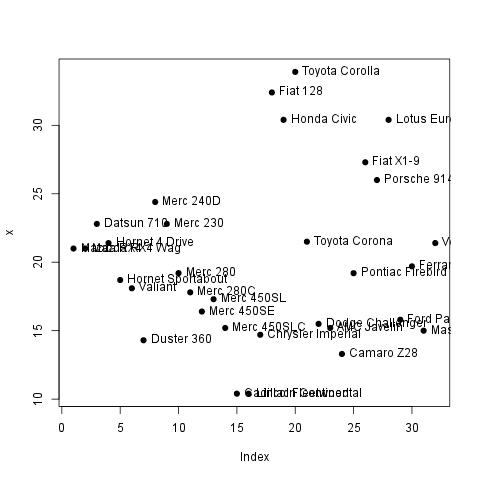
\includegraphics{bcc0dbaf4a393aacd8f480329c88e68f.png}
\caption{}
\end{figure}

So far we've been dealing with data.frames and plots, now let's deal
with variables

Now we'll see if the Z var is working properly. If I omit it, it should
perserve the default value (TRUE)\ldots{} aaaand\ldots{}. TRUE.

OK, so far, so good, but let's see what's going on with code
chunks\ldots{}

\ctable[pos = H, center, botcap]{llllllllll}
{% notes
}
{% rows
\FL
0.21696 & 0.50174 & 0.22349 & --2.49296 & 0.83943 & 0.92650 & 0.12971 & 0.28960 & 2.49944 & 0.70745
\\\noalign{\medskip}
--0.00474 & --0.44688 & 0.63431 & 0.16124 & 0.13629 & --1.68244 & --0.77522 & 0.04510 & --2.16911 & --1.36643
\\\noalign{\medskip}
--0.60781 & --0.49399 & --0.76930 & 1.15453 & --0.25689 & 1.10013 & --2.02654 & --0.19706 & 0.20225 & --1.49571
\\\noalign{\medskip}
0.15967 & --0.13376 & --0.01630 & --0.66398 & --1.34999 & 0.27609 & --1.59700 & --0.92464 & 1.22796 & 0.86069
\\\noalign{\medskip}
0.85585 & 1.98238 & 0.86331 & --0.58917 & --2.07967 & 0.35422 & --0.23036 & 0.56239 & --0.44610 & 0.41423
\\\noalign{\medskip}
0.44926 & --3.02493 & 0.16428 & --0.64600 & 1.01250 & --1.25318 & 0.00740 & 0.06426 & 0.30169 & 0.05773
\\\noalign{\medskip}
0.48462 & 1.18370 & --1.12861 & 0.76260 & --0.20068 & 0.82466 & 2.01900 & --1.11847 & 0.29299 & --0.80400
\\\noalign{\medskip}
0.38761 & --1.37269 & --0.73651 & --0.51947 & --0.52728 & --0.84735 & 0.85965 & 1.28130 & --0.96874 & --1.48523
\\\noalign{\medskip}
--0.52076 & 0.16741 & 1.61759 & --0.43654 & --0.85698 & --1.26634 & 0.09499 & 1.23600 & 0.04324 & 0.58843
\\\noalign{\medskip}
--1.93349 & 0.78008 & 0.56110 & 0.83768 & --0.67731 & 1.07995 & --0.39401 & --0.79811 & --1.18033 & 0.62871
\LL
}

When it comes to CSV values, let us see how do they work. You have
chosen the ``foo''.

\subsection{Description}

A simple report.

\subsubsection{Descriptive statistics}

The average fuel consumption is 146.69 with SD of 68.563. Let's add one
more line to this paragraph. And another one. Now, you've probably heard
of \emph{pi}? Right? Its value is 3.1416.

\subsubsection{Graphs}

And some graphs:

\begin{figure}[htbp]
\centering
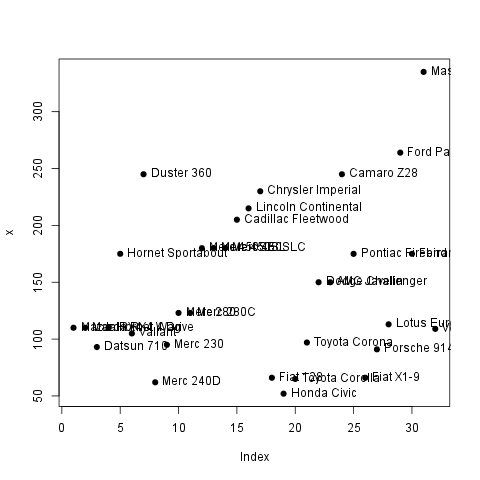
\includegraphics{31cfadc943dc05ceb88d3c07b411cf28.png}
\caption{}
\end{figure}

So far we've been dealing with data.frames and plots, now let's deal
with variables

Now we'll see if the Z var is working properly. If I omit it, it should
perserve the default value (TRUE)\ldots{} aaaand\ldots{}. TRUE.

OK, so far, so good, but let's see what's going on with code
chunks\ldots{}

\ctable[pos = H, center, botcap]{llllllllll}
{% notes
}
{% rows
\FL
0.22234 & 0.65173 & 1.39133 & 0.98333 & --0.58344 & --0.99095 & --0.45373 & --0.65796 & 2.37939 & 2.06748
\\\noalign{\medskip}
--0.31492 & --0.84771 & --0.55026 & 0.91617 & --0.16968 & 1.27141 & 0.46340 & --0.10636 & --0.18371 & --0.24102
\\\noalign{\medskip}
0.07103 & 0.00653 & --0.35326 & 0.81124 & 0.17430 & --0.15579 & --0.14371 & 1.03454 & --0.11201 & 0.77493
\\\noalign{\medskip}
0.85391 & --1.71403 & 0.53827 & 0.22948 & 0.32925 & --0.39897 & 1.07016 & --1.15996 & --0.04254 & 0.99816
\\\noalign{\medskip}
1.84811 & --1.97597 & 1.90410 & 0.29464 & --0.26010 & 0.05813 & --1.38199 & 0.54703 & --0.05245 & 0.24624
\\\noalign{\medskip}
--0.74688 & 1.50558 & --0.13179 & 1.68098 & 1.29912 & 0.21735 & 0.89660 & 0.09138 & --0.31560 & 0.93897
\\\noalign{\medskip}
--1.55898 & 3.47041 & 1.33684 & 0.26634 & --0.14000 & 0.42141 & --0.14711 & --0.91866 & --1.73281 & 0.48034
\\\noalign{\medskip}
--1.08743 & --0.62727 & 0.58817 & --1.52503 & --0.61666 & 0.03544 & --0.87532 & 0.41800 & --0.49410 & --0.47320
\\\noalign{\medskip}
--0.14827 & --0.08834 & --1.65963 & 0.34622 & 0.59807 & 0.13834 & 0.62300 & 0.74279 & 0.71904 & 1.04388
\\\noalign{\medskip}
--0.65230 & --0.71892 & --2.85295 & 0.08785 & --0.30507 & --1.72776 & 0.76428 & 1.77922 & 1.05258 & 1.01411
\LL
}

When it comes to CSV values, let us see how do they work. You have
chosen the ``foo''.

\subsection{Description}

A simple report.

\subsubsection{Descriptive statistics}

The average fuel consumption is 2.0628 with SD of 2.0404. Let's add one
more line to this paragraph. And another one. Now, you've probably heard
of \emph{pi}? Right? Its value is 3.1416.

\subsubsection{Graphs}

And some graphs:

\begin{figure}[htbp]
\centering
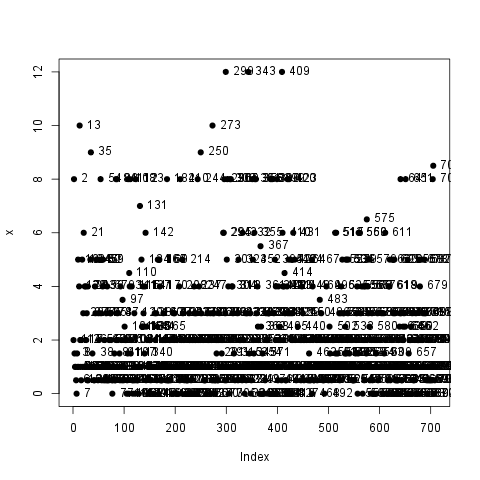
\includegraphics{a28c9526df56f14f4db444f97f519855.png}
\caption{}
\end{figure}

So far we've been dealing with data.frames and plots, now let's deal
with variables

Now we'll see if the Z var is working properly. If I omit it, it should
perserve the default value (TRUE)\ldots{} aaaand\ldots{}. TRUE.

OK, so far, so good, but let's see what's going on with code
chunks\ldots{}

\ctable[pos = H, center, botcap]{llllllllll}
{% notes
}
{% rows
\FL
1.72828 & 0.00902 & --0.42988 & --0.42918 & --0.31233 & 0.86316 & --0.76035 & 0.73025 & --1.29166 & 0.47547
\\\noalign{\medskip}
0.72337 & 1.48224 & --0.59635 & 0.10393 & 0.55306 & --0.45044 & --2.02105 & --0.57019 & 0.71030 & 1.13604
\\\noalign{\medskip}
1.22395 & 0.10938 & 0.38807 & --0.51683 & 1.79204 & --0.18481 & 0.40610 & --0.22629 & 1.32677 & --1.73743
\\\noalign{\medskip}
0.36481 & 2.31903 & 0.69694 & 0.54454 & 0.76660 & --1.21620 & --0.38909 & 0.46635 & --0.04112 & --1.84051
\\\noalign{\medskip}
--1.27903 & 0.73900 & --0.52441 & --1.00506 & 2.15166 & --0.92249 & --0.34753 & 0.97207 & 0.07277 & 1.82394
\\\noalign{\medskip}
0.05284 & 0.43922 & 0.01174 & 0.15163 & --1.51874 & --2.05551 & --0.51695 & --0.27935 & --0.26791 & 0.98499
\\\noalign{\medskip}
--0.27293 & 2.10518 & --1.91476 & --0.25366 & 0.32643 & 1.37410 & --0.33690 & 0.85166 & 0.02857 & --1.01447
\\\noalign{\medskip}
--0.08657 & 0.24202 & --0.58678 & --1.14747 & --1.78722 & --0.14218 & --1.70038 & 1.11414 & --1.02090 & 0.84343
\\\noalign{\medskip}
--1.14003 & 0.36409 & 0.14422 & 0.62636 & 1.81143 & 0.12810 & 0.45547 & 1.25006 & 0.61398 & --0.58169
\\\noalign{\medskip}
--0.81676 & 1.19413 & 0.96644 & 0.84559 & --0.48541 & 0.36482 & 0.77711 & --1.64583 & 0.28705 & --0.75663
\LL
}

When it comes to CSV values, let us see how do they work. You have
chosen the ``foo''.

\end{document}
